\documentclass[a4paper]{extarticle}
\usepackage[utf8]{inputenc}
\usepackage[a4paper, margin=1in]{geometry}

\usepackage{amssymb}
\usepackage{amsmath}
\usepackage{enumitem}
\usepackage{tcolorbox}
\usepackage{fancyhdr}
\usepackage{graphicx}
\usepackage{float}

\setlength{\parindent}{0em}
\setlength{\parskip}{0.4em}

\definecolor{theoremblue}{RGB}{1, 73, 124}
\definecolor{corollaryblue}{RGB}{70, 143, 175}
\definecolor{exampleblue}{RGB}{137, 194, 217}

\newtcolorbox{tbox}{colback=theoremblue!20,colframe=theoremblue,
boxrule=0pt,arc=0pt,boxsep=2pt,left=2pt,right=2pt,leftrule=2pt}

\newtcolorbox{cbox}{colback=corollaryblue!20,colframe=corollaryblue,
boxrule=0pt,arc=0pt,boxsep=2pt,left=2pt,right=2pt,leftrule=2pt}

\newtcolorbox{ebox}{colback=exampleblue!20,colframe=exampleblue,
boxrule=0pt,arc=0pt,boxsep=2pt,left=2pt,right=2pt,leftrule=2pt}

\title{IntroML - Lecture Notes Week 4}
\author{Ruben Schenk, ruben.schenk@inf.ethz.ch}
\date{\today}

\pagestyle{fancy}
\fancyhf{}
\rhead{ruben.schenk@inf.ethz.ch}
\rfoot{Page \thepage}
\lhead{IntroML - Lecture Notes Week 4}

\begin{document}

\maketitle
\newpage

\section{Classification}

\subsection{Classification Problem}

We start by comparing regression and classification:

\begin{itemize}
    \item \textbf{Regression:} Labeling \(x \to y \in Y\) where \(Y\) is a real value in \(\mathbb{R}\)
    \item \textbf{Classification:} Labeling \(x \to y \in Y\) where \(Y\) is a finite, discrete set, e.g. \(\{1, \, 2,..., \, K\}\) or \(\{-1, \, +1\}\).
\end{itemize}

For classification, inputs \(x\) and outputs \(y\) may look as follows:

\begin{table}[H]
    \centering
    \begin{tabular}{|l|l|}
        \hline
        \textbf{X}   & \textbf{Y}            \\ \hline
        Documents    & Sentiment (among $K$) \\ \hline
        Images       & Object (among $K$)    \\ \hline
        Emails       & Spam (yes or no)      \\ \hline
        Medical data & At risk (yes or no)   \\ \hline
    \end{tabular}
    \caption{Examples of classifications.}
    \label{tab:tb0401-classification}
    \end{table}

We distinguish the first two and the last two examples into \textit{multiclass classification} and \textit{binary classification.}

\subsection{Losses for Classification}

\subsubsection{Evaluation}

Again, we first introduce the \textbf{ML (Binary) Classification Pipeline:}

\begin{figure}[H]
    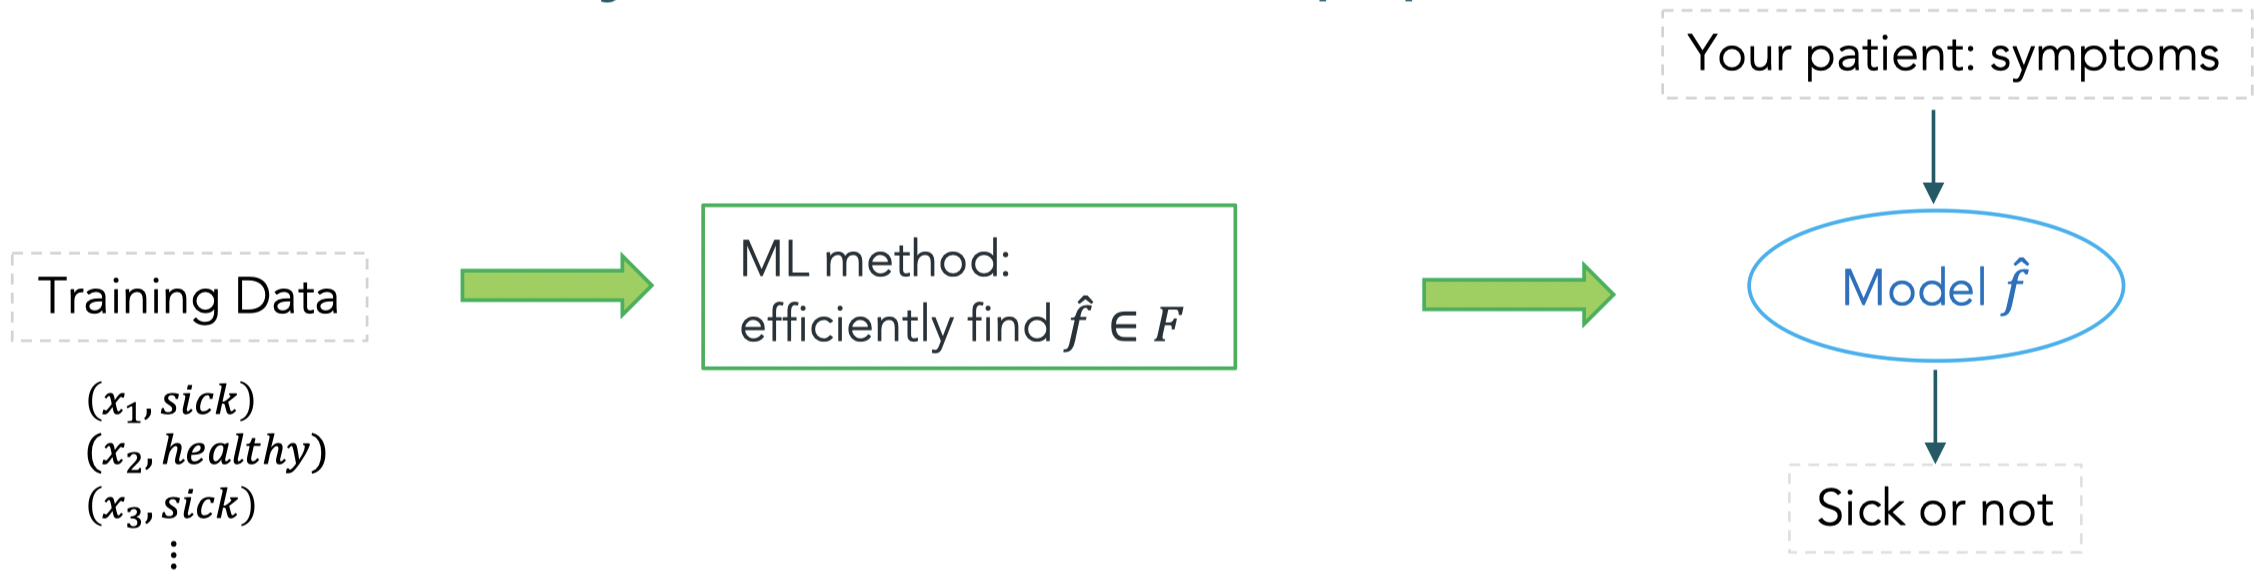
\includegraphics[width=15cm]{../images/IntroML_Fig4-1}
    \centering
\end{figure}

\textbf{Binary classification} is done using a function \(\hat{f} : \mathbb{R}^d \to \mathbb{R}\):

\begin{itemize}
    \item First, assign a number to the labels, for example "sick" = class 1, "healthy" = class 0
    \item One could choose these values at random w.l.o.g., but for binary classification it's often convenient to use +1 and -1
    \item Then, the predicted class is \(\hat{y} = \text{sign} \hat{f}(x)\)
    \item A \textit{good model} predicts \(\hat{y} = y\), where \(y\) is the true label
\end{itemize}

\begin{figure}[H]
    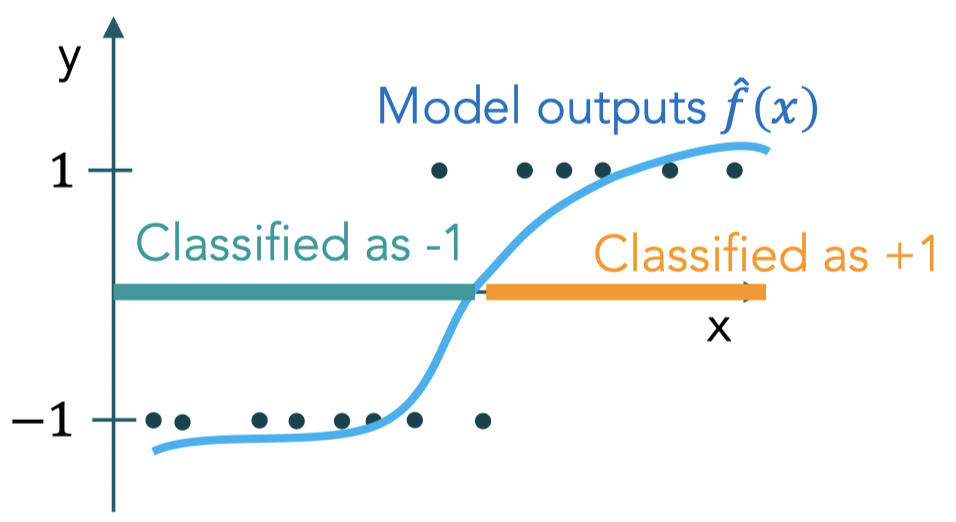
\includegraphics[width=6cm]{../images/IntroML_Fig4-2}
    \centering
\end{figure}

We have already seen that the \textbf{good model} in regression is determined by, given some data that follows the model \(y = f^*(x) + \epsilon = \langle w^*, \, x \rangle + \epsilon\) for some \(f^*\), the average prediction (generalization) error \(R(\hat{f}) := \mathbb{E}_{x, \, y}l(\hat{f}(x), \, y) = \mathbb{E}_{x, \, y}(\hat{f}(x), \, y)^2\).

How does the good model look like for classification? For data that follows the model, i.e. \(y = \epsilon \text{sign} f^*(x)\) with \(\epsilon \in \{-1, \, +1\}\) for some \(f^*\), we care about the \textbf{average classification (generalized) error:}

\[
    R(\hat{f}) := \mathbb{P}_{x, \, y}[y \neq \text{sign} \hat{f}(x)] = \mathbb{E}_{x, \, y} \mathbb{I}_{\{y \neq \text{sign} \hat{f}(x)\}} = \mathbb{E}_{x, \, y} l_{0-1}(\hat{f}(x), \, y),
\]

where \(l_{0 - 1}(\hat{f}(x), \, y) = \mathbb{I}_{\{y \neq \text{sign}\hat{f}(x)\}}\) is called the \textit{zero-one loss} and:

\[
    \mathbb{I}_{\{A\}} = \begin{cases}
        1, &A \text{ is true}, \\
        0, &A \text{ is false}.
    \end{cases}
\]

\subsubsection{Training and Surrogate Losses}

It is important to note that \textit{training loss is not equal to the evaluation loss.} We have a dichotomy betnween pointwise loss we care about when predicting during test time and the pointwise surrogate loss we might use to train our model!

\begin{figure}[H]
    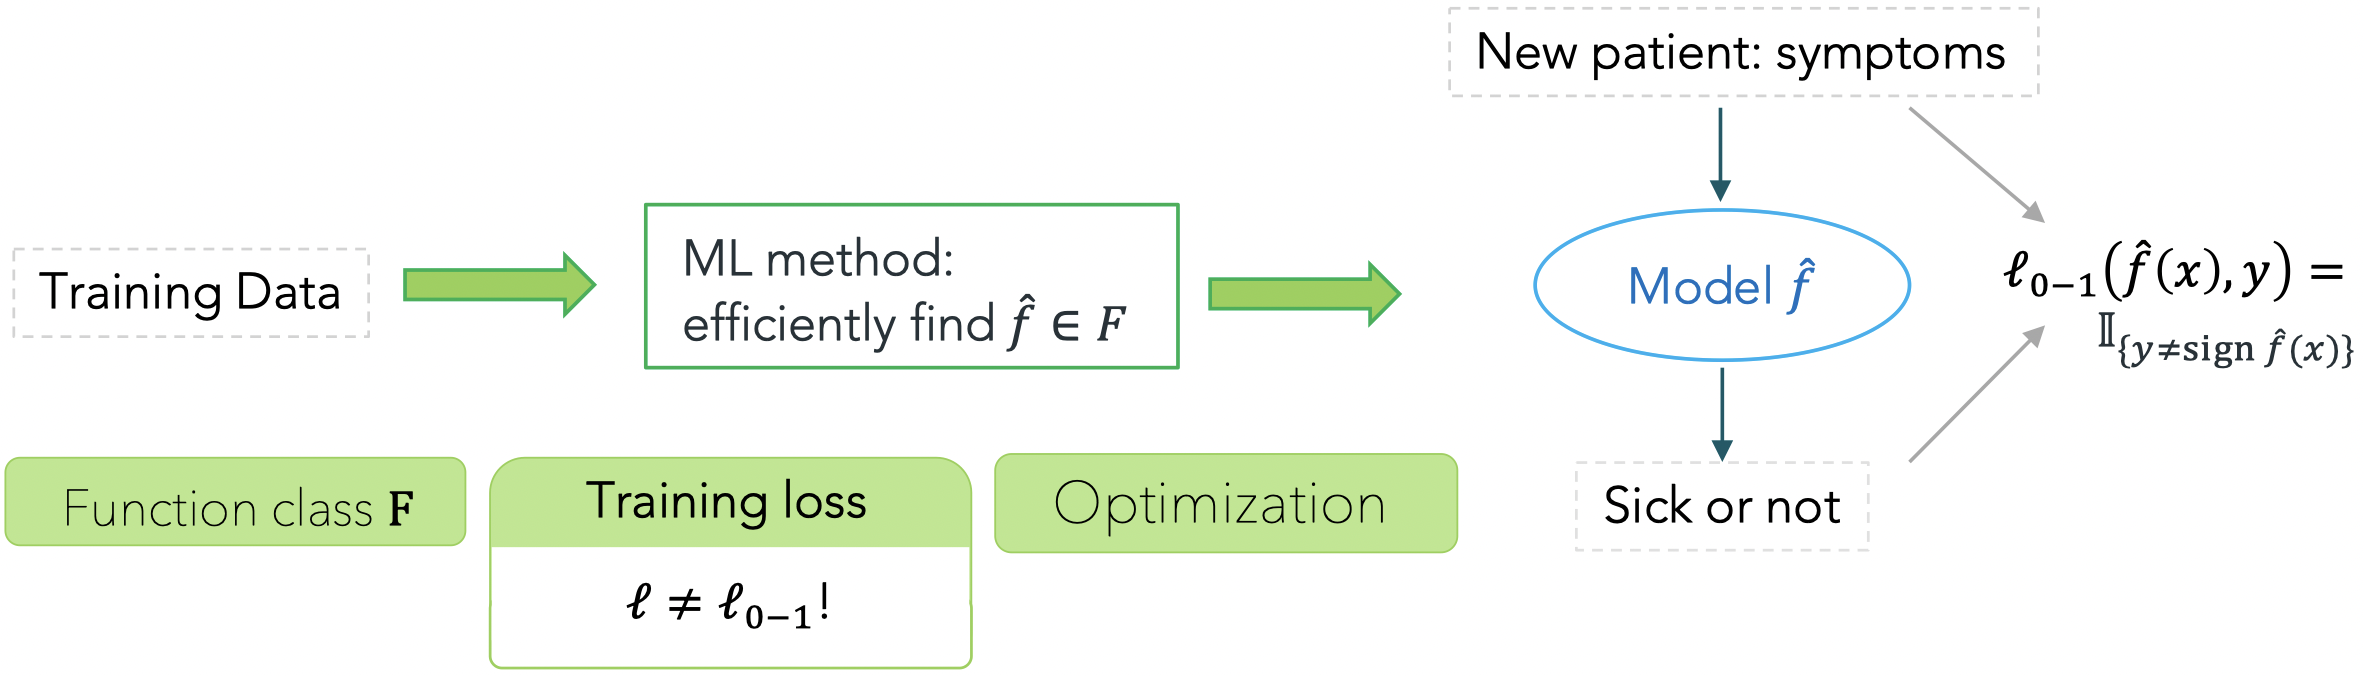
\includegraphics[width=15cm]{../images/IntroML_Fig4-3}
    \centering
\end{figure}

We would like a convex surrogate loss that also only depends on \(yf(x)\). In general, we need to penaltize when \(y\hat{f}(x)\) is small, or \(-y\hat{f}(x)\) is big, that is, the loss function should be of type \(l(\hat{f}(x), \, y) = g(y\hat{f}(x))\) for some \(g(z)\) that is large when \(z < 0\) and vice versa.

Therefore, in the following figure, only B and D would work:

\begin{figure}[H]
    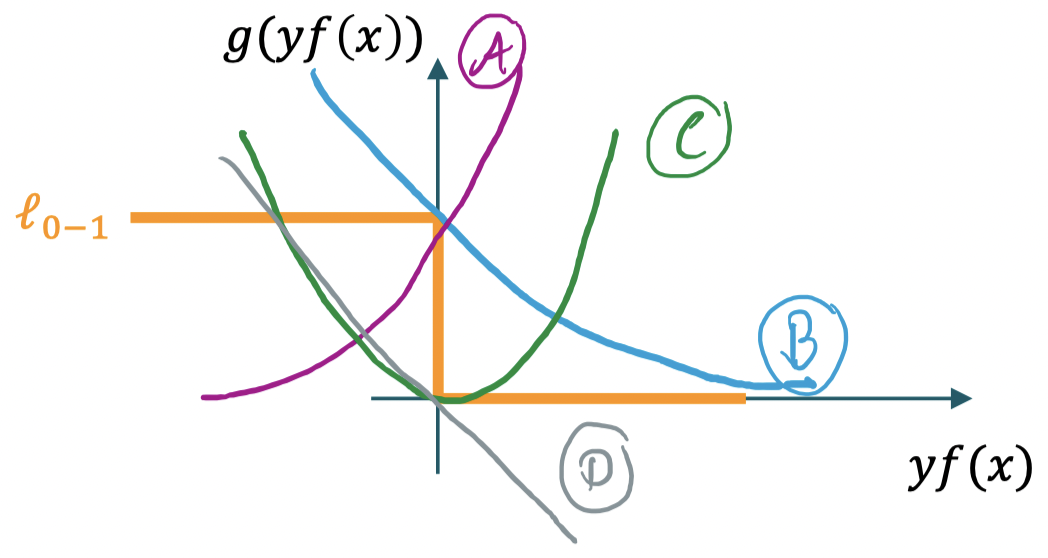
\includegraphics[width=6cm]{../images/IntroML_Fig4-4}
    \centering
\end{figure}

The following functions satisfy that \(g(y\hat{f}(x))\) is increasing in \(-y\hat{f}(x)\):

\begin{itemize}
    \item Exponential: \(g_{exp}(y \hat{f}(x)) = e^{-y \hat{f}(x)}\)
    \item Logistic: \(g_{log}(y \hat{f}(x)) = \log (1 + e^{-y \hat{f}(x)})\)
    \item Hinge: \(g_{hinge}(y \hat{f}(x)) = \max (0, \, 1 - y \hat{f}(x))\)
    \item Linear function: \(g_{lin}(y \hat{f}(x)) = -y\hat{f}(x)\)
\end{itemize}

\subsubsection{Logistic Loss}

We can rewrite \(\hat{y} = \text{sign}[\hat{f}(x)] = \arg \max_{c \in \{-1, \, +1\}} c\hat{f}(x)\) since \(\text{sign} \hat{f}(x) \cdot \hat{f}(x) \geq \hat{f}(x)\). If we assign \(0\) instead of \(-1\) for one of the classes, we can define vector \(\tilde{f}(x) := (- \hat{f}(x), \, \hat{f}(x))\) and then \(\hat{y} = \arg \max_i (\tilde{f}(x))_{[i]}\).

For any vector \(\tilde{f} \in R^K\) we define the \textbf{softmax} transformation \(\text{softmax} : R^K \to R^K\) to vector \(\hat{p} \in R^K\) as follows:

\[
    \hat{p}_{[i]} = (\text{softmax} (\tilde{f}))_{[i]} = \frac{\exp(\tilde{f}_{[i]}/2)}{\sum_{i = 1}^{K} \exp(\tilde{f}_{[i]}/2)}
\]

In particular, we can rewrite \(\hat{y} = \arg \max_i (\hat{p}(x))_{[i]}\).

Furthermore, note that \(\hat{p} = \text{softmax}(\tilde{f})\) is a probability vector, that is, \(\hat{p}_{[i]} \geq 0\) and \(\sum_{i = 0}^{K - 1} \hat{p}_[i] = 1\)! In particular, we can interpret \(\hat{p}_{[i]} = \text{Prob}(y = i)\). For binary, we use \(\hat{p}_0 = \text{Prob}(y = -1)\).

Using \(\hat{p}_0 = \frac{1}{1 + \exp(\hat{f}(x))}\) and \(\hat{p}_1 = 1 - \hat{p}_0\), we can now derive logistic loss from the 0-1 loss using "probabilistic" perspective of the softmax:

\[
    l_{log}(\hat{f}(x), \, y) = \mathbb{I}_{y = -1}\log(1 + e^{\hat{f}(x)}) + \mathbb{I}_{y = + 1}\log(1 + e^{- \hat{f}(x)}) = \log(1 + e^{-y\hat{f}(x)})
\]

\subsection{Linear Classifiers}

\textbf{Linear classifiers} are of the form

\[
    F = \{f : f(x) = w^Tx \text{ for some } w \in R^d\}
\]

Training and prediction is fairly simple! The decision boundary of a function \(f\) is \(\{x : f(x) = 0\}\). The prediction and 0-1 eroor only depends on \(\frac{w}{||w||}\) and uses \(\hat{y} = \text{sign} \hat{f}(x)\), training is done using \(\text{softmax}(\hat{f})\).

\begin{figure}[H]
    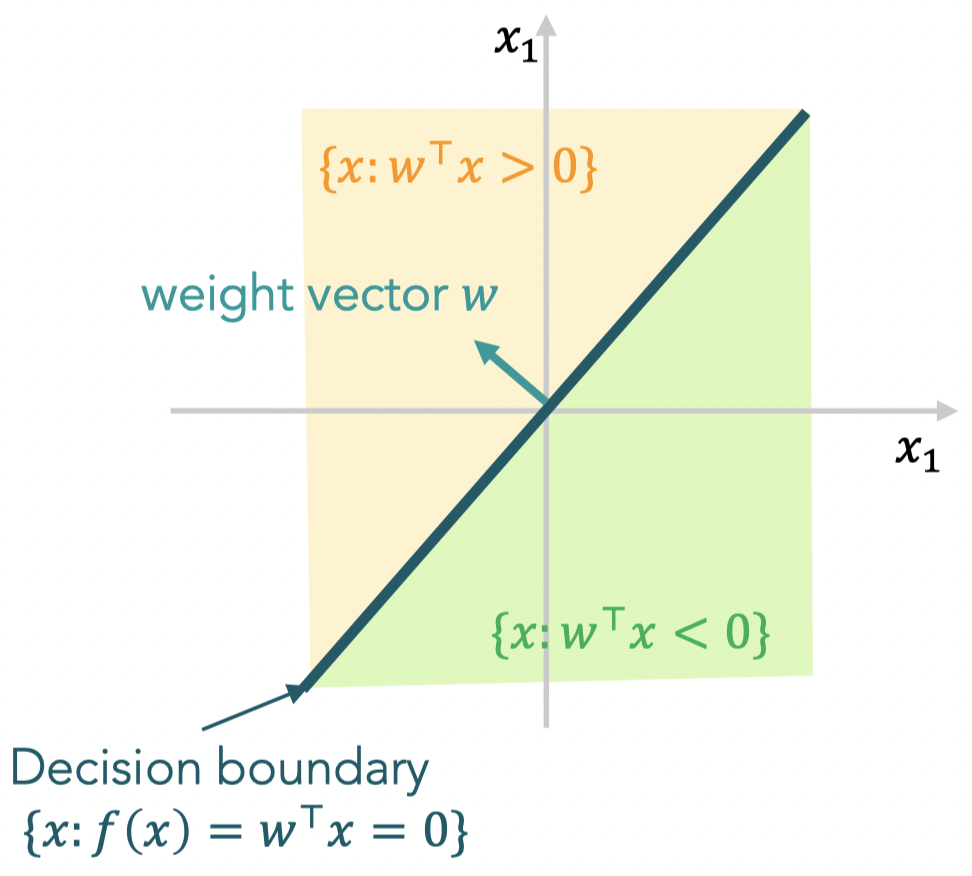
\includegraphics[width=6cm]{../images/IntroML_Fig4-5}
    \centering
\end{figure}

\subsubsection{Logistic Regression}

Recall the \textbf{logstic loss} to be \(l_{log}(f(x), \, y) = \log (1 + e^{-yf(x)})\).

For linear classifiers, the \textbf{training loss} is defined as \(L(w) = \frac{1}{n}\sum_{i = 1}^n \log(1 + e^{-y_iw^Tx_i})\) for the training points \(\{(x_i, \, y_i)\}_{i = 1}^n\).

Further, we consider linearly parameterized \(f_w(x) = \langle w, \, x \rangle\) and our gradient descent iterates are

\[
    w^{t + 1} = w^t - \eta \frac{1}{n} \sum_{i = 1}^n \nabla_w g(y \langle w^t, \, x \rangle) \nabla_w y \langle w^t, \, x \rangle
\]

We use the chain rule to compute \(\nabla_w g(y \langle w^t, \, x \rangle) = g'(y \langle w^t, \, x \rangle)\nabla_w y \langle w^t, \, x \rangle\). After that, the update reads

\[
    w^{t + 1} = w^t + \eta_t \frac{1}{n} \sum_{i = 1}^n \frac{y_ix_i}{1 + e^{y_iw^Tx_i}}
\]

Assuming linearly separable data, the gradient descent (initialized at 0) on the logistic loss converges to the direction \(w_{MM}\) that maximizes the minimum \(l_2\)-distance among all points. In particular, we can write \(w_{MM} = \arg \max_{||w||_2 = 1} \min_i y_i \langle w, \, x_i \rangle\).

\begin{figure}[H]
    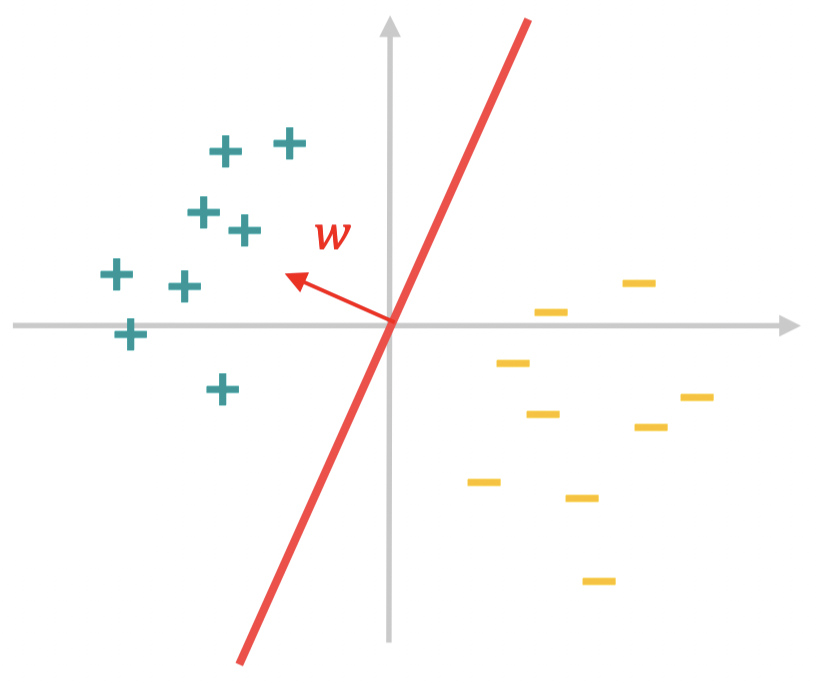
\includegraphics[width=6cm]{../images/IntroML_Fig4-6}
    \centering
\end{figure}

\subsubsection{Margin and Support Vector Machines}

The \textbf{max-margin direction} satisfies \(w_{MM} = \arg \max_{||w||_2 = 1} \min_i y_i \langle w, \, x_i \rangle =: \arg \max_{||w||_2 = 1} =\\ \text{margin}(w)\) and maximizes the minimum distance of points to the decision boundary \(\langle w, \, x \rangle = 0\).

For a general \(w\) that correctly separates the data, \(\frac{\text{margin}(w)}{||w||_2} = \frac{|w^Tx_i|}{||w||_2} = \frac{\text{margin}(\alpha w)}{||\alpha w ||_2}\), for any \(\alpha \in \mathbb{R}\), is the min. distance of any point to the boundary.

\begin{figure}[H]
    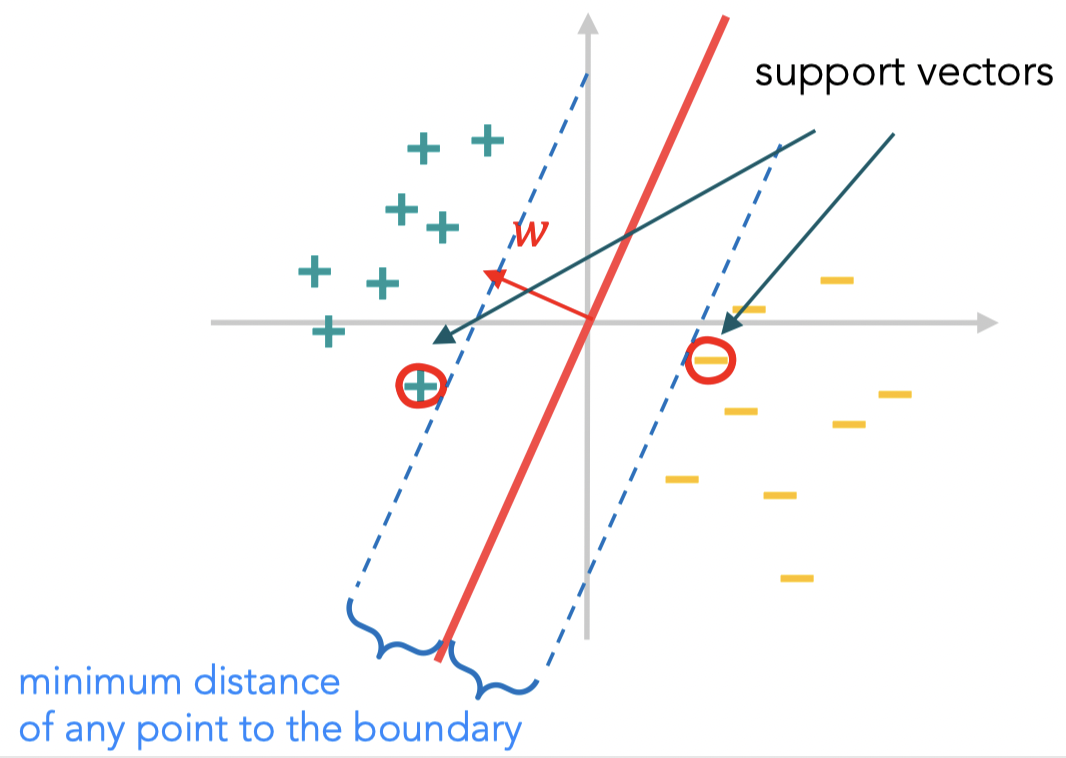
\includegraphics[width=6cm]{../images/IntroML_Fig4-7}
    \centering
\end{figure}

More generally, we cal also rewrite the optimization problem to:

\[
    w_{MM} || \arg \max_w \min_i y_i \langle \frac{w}{||w||_2}, \, x_i \rangle = \arg \max_w \frac{\text{margin}(w)}{||w||_2}
\]

We can rescale any unit norm \(w\) by \(\alpha = \frac{1}{\text{margin}(w)}\), i.e. \(\tilde{w} = \alpha w\) such that \(\text{margin}(\tilde{w}) = \min_i y_i \tilde{w}^Tx_i = \alpha \text{margin}(w) = 1\) with min. distance to dec. boundary \(\frac{\text{margin}(\tilde{w})}{||\tilde{w}||_2} = \frac{1}{||\tilde{w}||_2}\).

Hence, instead of searching within unit norm \(w\) to find \(w_{MM}\) with maximum min-distance \(\text{margin}(w)\), we can search within all \(\tilde{w}\) with \(\text{margin}(\tilde{w}) = 1\) to find the one that maximizes min-distance \(\)


\subsubsection{Multi-Class Classification}

\subsection{Non-Linear Classifiers}

\end{document}